% Danke AKM für das Template
\documentclass[11pt,a4paper]{article}
\renewcommand{\baselinestretch}{1.5}
\usepackage[utf8]{inputenc}
% Pakte für deutsche Begriffe
\usepackage[ngerman]{babel}
% Glossar und Abkürzungsverzeichnis
\usepackage[toc,acronym]{glossaries}
% Tabelle mit Zellen
\usepackage{makecell}
\usepackage[table]{xcolor}
\usepackage{subfigure}
\usepackage{xargs}
\usepackage{fixltx2e}
% Paket zum Einfügen der Fußzeilen
\usepackage[bottom]{footmisc}
% Paket zum Einfügen von URLs
\usepackage{url}
% setup for links
\usepackage[]{hyperref}
\hypersetup{hidelinks=true,}
% Pakete für das Einfügen von Bildern
\usepackage[pdftex]{graphicx}    
% Pfade angeben, in denen die Bilder sein könnten       
\graphicspath{./assets}    
% Dateiendungen für die Bilder      
\DeclareGraphicsExtensions{.pdf,.jpeg,.png,.jpg,.svg}
% Geometrie zum Erfüllen der IHK-Vorgabe 2,5cm Rand auf A4
\usepackage{geometry}
 \geometry{
  a4paper,
  total={170mm,257mm},
  left=25mm,
  right=25mm,
 }
\usepackage{caption}
% Zum Anzeigen der Tabelle- und Abbildungsverzeichnisse im Inhaltsverzeichnis
\usepackage[nottoc]{tocbibind}
%\usepackage{tocbibind}
% Zum Anhängen von PDF-Dokumenten
\usepackage[final]{pdfpages}

\usepackage{titlesec}


% Für Code-Block
\usepackage{listings}
\usepackage{color}
\definecolor{dkgreen}{rgb}{0,0.6,0}
\definecolor{gray}{rgb}{0.5,0.5,0.5}
\definecolor{mauve}{rgb}{0.58,0,0.82}
\lstset{frame=tb,
  language=bash,
  aboveskip=3mm,
  belowskip=3mm,
  showstringspaces=false,
  columns=flexible,
  basicstyle={\small\ttfamily},
  numbers=none,
  numberstyle=\tiny\color[HTML]{A3A1A8},
  keywordstyle=\color[HTML]{FF665A},
  commentstyle=\color[HTML]{7D6B7D},
  stringstyle=\color[HTML]{FF8C64},
  breaklines=true,
  breakatwhitespace=true,
  tabsize=3
}

\makeatletter
\AtBeginDocument{
  \hypersetup{
    pdftitle = {\@title},
    pdfauthor = {\@author}
  }
}
\makeatother
\author{Nico Kahlert}
\title{
  Einrichtung einer verteilten Monitoringlösung auf Basis von Prometheus und M3 
  im Bereich des behördlichen Gesundheitswesens
}

% Alle Glossareinträge
\makenoidxglossaries
\newglossaryentry{itz}
{
	name=ITZBund,
	description={Eine Behörde, welche IT-Dienstleistungen für staatliche Behörden der Bundesregierung erbringt \cite{itz}},
}
\newglossaryentry{bmg}
{
  name=Bundesministerium für Gesundheit,
  description={Eine Behörde auf Bundesebene mit dem Zuständigkeit für das deutsche Gesundheitswesen \cite{bundesgesundheitsministerium}},
}
\newglossaryentry{cdu}
{
  name={Christlich Demokratische Union},
  description={Eine christdemokratische Partei aus Deutschland, im politischen Spektrum mitte-rechts angeordnet}
}
\newglossaryentry{coronakrise}
{
  name=Coronakrise,
  description={
    Begriff der Medien für die soziale und ökonomische Krisensituation in Folge 
    der pandemische Ausbreitung des 2019 entdeckten Coronavirus SARS-CoV-2
  },
}
\newglossaryentry{pandemiemanagementsoftware}
{
  name=Pandemiemanagementsoftware,
  description={
    Softwaresystem zur Unterstützung des Gesundheitssystems im Zuge von Kontaktverfolgung, Quarantänemanagement etc
  },
}
\newglossaryentry{itil}
{
  name={ITIL},
  description={
    Leitfaden und Standard im IT-Service-Management
  },
}
\newglossaryentry{Availability Management}
{
  name={Availability Management},
  description={
    Ein Unterpunkt von \gls{itil} bei dem die Verfügbarkeit eines Dienstes anhand 
    von Qualitätsparametern definiert wird
  },
}
\newglossaryentry{docker}
{
  name={Docker},
  description={
    Ein Unternehmen, welches die gleichnamige OpenSource Containerruntime entwickelt und Softwarecontainerisierung
    in das betriebliche Standardportfolio einführte \cite{docker}
  },
}
\newglossaryentry{day2ops}
{
  name={Day2Ops},
  description={
    Ein zusammenfassender Begriff für alle Operationen, welche nach der Inbetriebnahme von Softwaresystemen
    ausgeführt werden. Eingeführt wurde der Begriff von der Firma D2IQ (ehemals Mesosphere) \cite{d2}
  },
}
\newglossaryentry{microservice}
{
  name={Microservice},
  description={
    Eine Softwarearchitektur, in welcher ein Dienst aus mehreren kleineren Diensten gebildet wird,
    welche jedoch unabhängig voneinander betrieben werden können. Es wird so erhofft, weniger
    Entwicklungsbedarf und bessere Lesbarkeit des Quellcodes zu erreichen \cite{ms}
  },
}
\newglossaryentry{whiteboxmonitoring}
{
  name={Whiteboxmonitoring},
  description={
    Eine Monitoringpraxis, wobei die zu monitorende Applikation selbst die eigenen Betriebsdaten
    für das Monitoringsystem bereitstellt \cite{sre}
  },
}
\newglossaryentry{go}
{
  name={Golang},
  description={
    Eine bei Google unter anderem von Ken Thompson entwickelte statischtypisierte Systemprogrammiersprache mit
    einer automatischen Speicherbereinigung (Garbage Collection) und Schwerpunkt auf einen minimalen Syntax 
    basierend auf der Sprache C \cite{go}
  },
}
\newglossaryentry{exporter}
{
  name={Metricsexporter},
  description={
    Ein Programm zum Sammeln von Betriebsdaten und Übertragung in Prometheusmetriken,
    welche von einem \gls{http}-Endpunkt abgerufen werden können \cite{exporter}
  },
}
\newglossaryentry{timeseries}
{
  name={Timeseries},
  description={
    Eine nach Zeitpunkten indizierte Serie von Datenpunkten
  },
}
\newglossaryentry{DSL}
{
  name={Domain Specific Language},
  description={
    Eine nach Zeitpunkten indizierte Serie von Datenpunkten
  },
}
\newglossaryentry{YAML}
{
  name={YAML},
  description={
    Eine einfache Datenbeschreibungssprache, bei der die Einrückung die Datenstruktur wiedergibt
  },
}
\newglossaryentry{JSON}
{
  name={JSON},
  description={
    Eine einfache Datenbeschreibungssprache mit dem Ursprung aus der Notation von JavaScript Objekten
  },
}
\newglossaryentry{cassandra}
{
  name={Cassandra},
  description={
    Eine bei Facebook entwickelte, freie und OpenSource NOSQL-Datenbank. Cassandra wird meistens verteilt
    betrieben und macht dies durch eine \emph{Distributed Hashtable (DHT)} möglich. Die Daten werden als
    \emph{Spalten} in Tabellen organisiert dargestellt und können mittels der \emph{Cassandra Query Language (CQL)}
    abgefragt werden \cite{cassandra}
  },
}
\newglossaryentry{NOSQL}
{
  name={NOSQL},
  description={
    Ein Überbegriff für alle Datenbankkonzepte, die nicht dem relationalem SQL-Ansatz folgen \cite{nosql}
  },
}
\newglossaryentry{CAP}
{
  name={Brewers Theorem},
  description={
    Sagt aus, dass die Garantie, in einer verteilten Software Ausfalltoleranz, Verfügbarkeit und Konsistenz
    gleichermaßen zu berücksichtigen, nicht möglich ist \cite{cap}
  },
}
\newglossaryentry{namespaces}
{
  name={Namespaces},
  description={
    Höchste Abstraktionseinheit der M3DB. Vergleichbar mit den Datenbanken der relationalen Datenbankmanagementsoftware
  },
}
\newglossaryentry{shards}
{
  name={Shard},
  description={
    Eine virtuelle Einheit der M3DB, in welcher Timeseriesschlüssel \glsadd{timeseries} auf einen Knoten zugewiesen werden 
  },
}
\newglossaryentry{etcd}
{
  name={ETCD},
  description={
    Ein weitverbreiteter verteilter Key-Value-Store basierend auf dem Consensusprotocol \emph{RAFT} \cite{etcd}
  },
}
\newglossaryentry{Protobuf}
{
  name={Protocolbuffer},
  description={
    Ein von Google entwickelter Standard zur nachhaltigen Darstellung von Daten im Binärformat
  },
}
\newglossaryentry{SSH}
{
  name={SSH},
  description={
    Ein Netzwerkprotokoll zur verschlüsselten Kommunikation über Netzwerke. Meist wird das 
    Protokoll für die Verbindung auf das Terminal eines Servers verwendet. Die bekannteste Implementation 
    ist die freie Software \emph{OpenSSH}. Die Portnummer von SSH ist die 22
  },
}
\newglossaryentry{daemon}
{
  name={Daemon},
  description={
    Eine etablierte Bezeichnung für Server- oder Hindergrundprozesse auf UNIX und seinen Nachfolgern
  },
}
\newglossaryentry{python}
{
  name={Python},
  description={
    Eine beliebte objektorientierte, dynamischtypisierte Skriptsprache mit einfachem Syntax
  },
}
\newglossaryentry{playbooks}
{
  name={Playbooks},
  description={
    Eine oder mehrere Dateien im \gls{YAML}-Format, welche den Zielzustand eines von Ansible verwalteten Systems
    beschreiben
  },
}
\newglossaryentry{rollen}
{
  name={Rollen},
  description={
    Ein hierarchisch untergeordneter Teil eines \gls{playbooks}, welcher zur Übersichtlichkeit und Wiederverwendbarkeit
    von Code eines Ansibleprojektes beitragen sollen
  },
}
\newglossaryentry{inventory}
{
  name={Inventory},
  description={
    Eine Liste von Severn im \gls{YAML}- oder \gls{INI}-Format für die Verwaltung mit Ansible.
    Server können auch gruppiert werden
  },
}
\newglossaryentry{INI}
{
  name={INI},
  description={
    Ein menschenlesbares, einfaches Textformat, bei dem Daten als Schlüssel-Werte-Paare formatiert sind
  },
}
\newglossaryentry{SPoF}
{
  name={Single Point of Failure},
  description={
    Ein Teil eines Systems, welches keine Ausfalltoleranz aufweist
    und das gesamte System gefährden kann
  },
}
\newglossaryentry{images}
{
  name={Containerimages},
  description={
    Ein für Softwarecontainer verwendetes unveränderliches Paketformat mit den Dateien der Anwendungen und der 
    Laufzeitumgebung
  },
}
\newglossaryentry{raft}
{
  name={RAFT},
  description={
    Ein Konsensalgorithmus mit dem Ziel der einfachen Verständlichkeit \cite{raft}
  },
}
\newglossaryentry{splitbrain}
{
  name={Split-Brain},
  description={
    Ein Problem in Computerclustern mit gerader Knotenanzahl, bei dem die Knoten in gleichgroße Gruppen
    aufgetrennt werden und keine Mehrheit für die  Aufrechterhaltung der Konsistenz gebildet werden kann (siehe \gls{CAP}) \cite{split-brain}
  },
}
\newglossaryentry{remote}
{
  name={Remoterepository},
  description={
    Im Netzwerk oder Online vorbehaltene Kopien eines git-Repository
  },
}
\newglossaryentry{task}
{
  name={Task},
  description={
    Eine Anforderung an ein System, die Ansible ausführen soll und kleinste Einheit eines \gls{playbooks}
  },
}
\newglossaryentry{make}
{
  name={Make},
  description={
    Ein im Unixumfeld weitverbreitetes Werzeug zum Management und Vereinfachen
    von Softwarebuilds (wie Kompilierung und Linken von Programmen in C)
  },
}
% Alle Abkürzungen
\newacronym[see={[Glossar:]{bmg}}]{BMG}{BMG}{Bundesministerium für Gesundheit\glsadd{bmg}}
\newacronym[see={[Glossar:]{cdu}}]{CDU}{CDU}{Christlich Demokratische Union  \glsadd{cdu}}
\newacronym[see={[Glossar:]{itz}}]{ITZ}{ITZBund}{Informationstechnikzentrum Bund \glsadd{itz}}
\newacronym[see={[Glossar:]{pandemiemanagementsoftware}}]{sormas}{SORMAS}
  {''Surveillance Outbreak Response Management and Analysis System'' \glsadd{pandemiemanagementsoftware}}
\newacronym[]{netzlink}{Netzlink}{Netzlink Informationstechnik GmbH}
\newacronym[see={[Glossar:]{itil}}]{ITIL}{ITIL}{Information Technology Infrastructure Library \glsadd{itil}}
\newacronym[]{hzi}{HZI}{Helmholtz Zentrum für Infektionsforschung}
\newacronym[]{cncf}{CNCF}{Cloud Native Computing Foundation}
\newacronym[]{ebnf}{EBNF}{extended Backus-Naur Form}
\newacronym[]{http}{HTTP}{Hypertext Transfer Protocol}
\newacronym[]{rest}{REST}{Representational State Transfer}
\newacronym[]{promql}{PromQL}{Prometheus Query Language}
\newacronym[see={[Glossar:]{DSL}}]{dsl}{DSL}{Domain Specific Language \glsadd{DSL}}
\newacronym[see={[Glossar:]{YAML}}]{yaml}{YAML}{YAML \glsadd{yaml} Aint Markup Language \glsadd{YAML}}
\newacronym[see={[Glossar:]{JSON}}]{json}{JSON}{JavaScript Object Notation \glsadd{JSON}}
\newacronym[see={[Glossar:]{SSH}}]{ssh}{SSH}{Secure Shell \glsadd{SSH}}
\newacronym[]{vm}{VM}{virtuelle Maschine}
\newacronym[]{ssd}{SSD}{Solid State Drive}
\newacronym[]{saas}{SaaS}{Software as a Service}
% Alle renew - Commands
% Umbenennen des Abkürzungsverzeichnis
\renewcommand*{\acronymname}{Abkürzungsverzeichnis}
% Formatierungen der Zellen-Tabelle
\renewcommand\theadalign{bc}
\renewcommand\theadfont{\bfseries}
\begin{document}
\renewcommand{\familydefault}{\sfdefault}
\fontfamily{phv}\selectfont

% Deckblatt
\begin{titlepage}
  \vspace*{1cm}
  \begin{center}
    {\bfseries\Huge
      Einrichtung einer verteilten Monitoringlösung auf Basis von Prometheus und M3
      im Bereich des behördlichen Gesundheitswesens
    }
    \Large
    \vspace{1cm}

    Projektbericht\\
    von Nico Kahlert\\
    26.02.2021

    \begin{center}

      \begin{figure}[ht]
        \centering
        \includegraphics[width=7cm]{assets/ihk-logo.png}\\
        \includegraphics[height=1.25cm]{assets/netzlink.png}
      \end{figure}

    \end{center}
  \end{center}
  \begin{Large}
    \begin{tabular}{@{}ll}
      \textbf{Ausbildungsberuf:}      & Fachinformatiker für Systemintegration \\
      \textbf{Durchführungszeitraum:} & 26.02.2021 - 28.04.2021                \\
      \textbf{Verfasser / Prüfling:}  & Nico Kahlert                           \\
      \textbf{Prüfung:}               & Sommer 2021                            \\
      \textbf{Identnummer:}           & 594872                                 \\
      \textbf{Prüflingsnummer:}       & 111 3188                             \\
      \textbf{Ausbildungsbetrieb:}    & Netzlink Informationstechnik GmbH      \\
                                      & Westbahnhof 11                         \\
                                      & 38118 Braunschweig
    \end{tabular}
  \end{Large}
\end{titlepage}

% Vorwort ...
\pagenumbering{gobble}
\section*{Vorwort}
Um in diesem Bericht von der Wiedergabe von Rollenklischees und Stereotypen abzusehen,
wird von der Nutzung des generischen Maskulinum abgesehen und stattdessen ein sogenanntes
Gendersternchen zur Inklusion aller Geschlechtsidentitäten verwendet.
Weiterhin sind komplett großgeschriebene Wörter im Glossar erläutert.
Bedeutungsvolle Begriffe sind kursiv geschrieben.
Grafische Schaubilder und Diagramme befinden sich separiert im Anhang und werden im Text mittels
Verweis gekennzeichnet. Die in dem Bericht wiedergegebenen Projektphasen werden mit horizontalen Linien gekennzeichnet.
Die Farben dieser Linien entsprechen denen der Tabellen (Seite \pageref{table:gantt}).
\newpage

% Inhaltsverzeichnis ohne Seitenzahl
\thispagestyle{empty}
\pagenumbering{gobble}
\tableofcontents

\clearpage
\pagenumbering{arabic}
\setcounter{page}{1}
\fontfamily{phv}\selectfont
\section{Einleitung}
Im Zuge der andauernden \GLS{coronakrise}
wurde der Auftrag zum Betrieb der \gls{pandemiemanagementsoftware} \gls{sormas} in den Rechenzentren
des \gls{itz} an die \gls{netzlink} erteilt.
Aufgrund eines raschen Anstiegs von zu überwachenden Maschinen in unserer Infrastruktur
im Rechenzentrum des \GLS{itz} stellte sich heraus, dass die derzeitige Monitoringlösung
der Aufgabe nicht mehr standhalten kann. Diese Infrastruktur ist für die alleinige Überwachung
der dortigen Systeme verantwortlich, welche eine \emph{\gls{saas}} des behördlichen Gesundheitswesen
bereitstellen und als eine sogenannte \emph{kritische Infrastruktur} eingestuft werden.
Zur Verbesserung muss ein passendes Monitoringkonzept erarbeitet werden.
Dieser Entwicklungsbedarf und die Umsetzung des Projektes wird in dieser Dokumentation ganzheitlich
beschrieben.
\subsection{Vorstellung des Kunden}
Das \gls{BMG} ist vor allem zuständig für die Erarbeitung von Gesetzentwürfen
für das deutsche Gesundheitssystem und wird von der*m Bundesminister*in für Gesundheit geleitet.
Zur Zeit ist dies Jens Spahn von der \gls{CDU}.
Dem \gls{BMG}, welchem jährlich ungefähr 15 Milliarden Euro
Haushalt zur Verfügung steht, gehören circa 700 Bedienstete an. Es ist die höchste Instanz im Gesundheitssystem und
unter anderem als Akteur wegweisend in der Krankheitsprävention \cite{bundesgesundheitsministerium}.
\subsection{Projekteinordnung}
Da es sich beim Betrieb von \gls{sormas} für die behördlichen Gesundheitsämter um eine kritische Infrastruktur handelt,
muss zu jedem Zeitpunkt sichergestellt werden, dass der Dienst voll funktionsfähig ist. Die Basis dafür
ist ein Monitoringsystem, welches die Anforderungen an Stabilität und Strapazierfähigkeit unterstützt
und so eine dauerhafte Serviceüberwachung möglich macht. Im Leitfaden für IT-Service-Management \GLS{itil},
nach welchem der Service von \gls{netzlink} strukturiert ist, ist das Monitoring eine wichtige Datenquelle für das
\emph{\gls{Availability Management}} und somit ein Indikator für die Zufriedenheit des Kunden \cite{itil}.
\subsection{Auswahl des Projektes}
Die meiste Zeit verbrachte ich im OpenSolutions-Team, welches für den Betrieb und Architektur von OpenSource-Software bei Kund*innen
zuständig ist. Aus diesem Grund wollte ich auch das Abschlussprojekt in diesem Bereich durchführen.
\subsection{Verwendete Software}
Im Folgenden werden die Anwendungsbereiche der in der Umsetzung verwendeten Softwareprodukte beschrieben.
\subsubsection{Sormas}
\label{sssec:sormas}
\gls{sormas} ist eine Software zum Pandemiemanagement \glsadd{pandemiemanagementsoftware} und wurde vom \gls{hzi} aus Braunschweig
zusammen mit der Firma Vitagroup für die Ebola-Epidemie von Ostafrika 2014
entwickelt. In Folge der \gls{coronakrise} wird diese Webanwendung für den behördlichen Gesundheitsdienst
im Auftrag des \gls{BMG} von \gls{netzlink} im Rechenzentrum des \gls{itz} betrieben.
Gesundheitsamtsmitarbeiter*innen nutzen sie zur Nachverfolgung
von Kontakten und Quarantänezeiträumen. Die Software ist unter
der Apache OpenSource-Lizenz geschützt und kann von jeder*m frei betrieben werden. Geschrieben ist die Applikation
in Java und speichert ihre Daten in einer relationalen Postgresdatenbank. Die Software wird in Produktion bei \gls{netzlink}
in \gls{docker}-Containern betrieben, um ein möglichst leichtes Lifecyclemanagement und problemlose \gls{day2ops} zu garantieren.
Aktuell wird je Gesundheitsamt eine \gls{sormas}-Instanz inklusive Datenbank und Proxy auf einer virtuellen Maschine ausgerollt. \cite{sormas-oegd}
\subsubsection{Prometheus}
\label{sssec:prometheus}
Prometheus ist ein freies OpenSource Programm, welches ursprünglich bei dem in den USA ansässigen Streamingunternehmen
Soundcloud entwickelt wurde. Es dient dem Sammeln, Aggregieren, Speichern und Abfragen von Betriebsdaten von Sofwaresystemen.
Als Grundlage für das Sammeln der Daten dient das prometheuseigene, auf der \gls{ebnf} basierte Datenformat in Textform
(siehe Abbildung \ref{figure:metrics} auf Seite \pageref{figure:metrics}).
In einem typischen \gls{whiteboxmonitoring}szenario werden diese Daten, welche auch als Metriken bezeichnet werden,
über einen \gls{http}-Endpunkt mit dem Pfad \emph{/metrics} bereitgestellt.
Diese werden in regelmäßigen, einstellbaren Abständen von dem Prometheusserver abgegriffen (scraping) und auf dessen lokalen
Filesystem persistiert. Es ist auch möglich, externe \gls{timeseries}datenbanken mittels des \emph{Prometheusremoteprotocols}
zu nutzen. Die Metriken können über die \gls{rest} API oder der Weboberfläche abgegriffen werden.
Zum Einholen der Metriken wird die \gls{dsl} \gls{promql} verwendet \cite{prometheus}
(siehe Abbildung \ref{figure:promql} auf Seite \pageref{figure:promql}).
Innerhalb von \glsadd{docker} containerbasierten \gls{microservice}infrastrukturen gilt Prometheus im Verbund mit Grafana als Standard.
\subsubsection{Nodexporter}
\label{sssec:nodexporter}
Der Nodexporter ist ein in \gls{go} entwickelter \gls{exporter} zum Sammeln von Betriebsdaten des
darunterliegenden Betriebsystems. Das Programm zählt zu den Standardwerkzeugen der Monitoringlösung um Prometheus \cite{exporter}.
\subsubsection{Grafana}
\label{sssec:grafana}
Grafana ist ein universelles, webbasiertes Werkzeug zur grafischen Darstellung von Daten in Dashboards.
Es ist der Standard zur Visualisierung von \gls{promql}-Abfragen. Zur vereinfachten Integration der Dienste bietet
Grafana einen grafischen Integrationsworkflow für Prometheus \cite{grafana}.
\subsubsection{M3DB}
\label{sssec:m3db}
M3DB ist eine quelloffene verteilte \gls{timeseries}datenbank, welche bei dem Onlinevermittlungsunternehmen für
Personenbeförderung von Privatpersonen Uber als Alternative zur Datenbank \gls{cassandra} entwickelt wurde \cite{m3db}.
Sie ist in der Programmiersprache \gls{go} verfasst und basiert auf einem \gls{NOSQL} Modell. M3DB ist nach dem \gls{CAP}
als eine \emph{CP}-Datenbank \cite{cap} einzuordnen, da sie eine Ausfalltoleranz mit dem Replikationfaktor
\begin{math}
  RF = (N / 2) + 1
\end{math} (Wobei N die Anzahl der Knoten ist) arbeitet und verschiedene garantierte Konsistenzlevel anbietet.
Im Hintergrund verwendet die Datenbank ein externes oder eingebettetes \gls{etcd}-Cluster, in welchem
die Konfiguration von \emph{Clustermembership}, \gls{namespaces} und Platzierung von \gls{shards} stattfindet.
Die Datenbank implementiert außerdem
die Funktion eines \emph{Prometheusremoteprotokollendpunketes} zur Benutzung als \gls{timeseries}datenbank für Prometheus.
Das Management der Datenbank ist über eine \gls{rest}-API möglich.
Die Daten werden von der M3DB in Dateien auf dem Filesystem als sogenannte \emph{Filesets} im eigenen M3TSZ und \gls{Protobuf}format persistiert.
Diese Filesets werden sowohl für die auf Snapshots des \verb|B+-Tree| basierte Storageebene als auch für die Commitlogs verwendet.
Nach eigenen Aussagen konnten die gesamten Ausgaben des Monitorings bei Uber durch den Wechsel auf M3DB von zehn auf zwei Prozent
reduziert werden \cite{m3db-blog}.
\subsubsection{Consul}
\label{sssec:consul}
Consul ist eine von HashiCorp entwickelte verteilte Lösung zur Servicediscovery. Es beinhaltet die Möglichkeit, Dienste
über einen internen DNS-Server oder die \gls{rest}-API abzugreifen. Zur einfachen Visualisierung bietet es eine Weboberfläche.
\subsubsection{Ansible}
\label{sssec:ansible}
Ansible ist eine von Red Hat entwickelte Lösung zur Automatisierung und einfachen Orchestrierung von
IT-Systemen. Es basiert auf einem deklarativen Ansatz, bei welchem der gewünschte Zustand einer Umgebung
abstrahiert beschrieben wird. Der Ansibleprozess setzt dann Änder- ungen implizit auf den Zielsystemen meist über eine
einfache \gls{ssh}-Verbindung um, so dass oftmals keine weitere Software als \gls{daemon} auf den Zielhosts installiert sein muss.
Die Funktionen von Ansible können über Module in \gls{python} erweitert werden. Die Informationen über den Zielzustand des Systems
werden in einer oder mehreren Dateien im \gls{YAML}-Format, sogenannten \gls{playbooks}, beschrieben (siehe Abbildung \ref{figure:inv} auf Seite \pageref{figure:inv}).
Um Wiederverwendbarkeit und eine gute Codeübersicht zu garantieren, können Teile eines \gls{playbooks} in sogenannte \gls{rollen} gebündelt werden.
Diese haben das gleiche Format wie \gls{playbooks}, sind jedoch, im Gegenteil zu jenen, einer festen Ordnerstruktur unterworfen.
Die von Ansible verwalteten Server werden in einem \gls{inventory} verwaltet, welches als Liste von Servern im \gls{INI}- oder \gls{YAML}-Format
vorliegt (siehe Abbildung \ref{figure:ansible-inv} auf Seite \pageref{figure:ansible-inv}). \cite{ansible}
\\\noindent{\color[HTML]{FFF587} \rule{\linewidth}{1mm}}
\section{Projektplanung}
\subsection{Wirtschaftliche Betrachtung}
Da es sich bei allen Produkten um freie OpenSource-Software handelt, musste ich keine
kostenpflichtigen Lizenzen zum Einkauf übermitteln. Außerdem wurden die
benötigten virtuellen Maschinen vom Bund bereitgestellt. Somit werde ich lediglich
die beteiligten Mitarbeiter in die wirtschaftliche Betrachtung einfließen lassen
\emph{(siehe Tabelle \ref{table:aufwand} auf Seite \pageref{table:aufwand})}.
\subsection{Projektschnittstellen}
Die Bereitstellung der virtuellen Maschinen, inklusive des Betriebsystems,
wurde von den zu- ständigen Projektteams des \gls{itz} durchgeführt.
Dies gilt auch für sämtliche Konfigurationen im Bereich
der Netzwerke und Firewalls außerhalb der virtuellen Host
und ist nicht Teil des Projekts.
\subsection{Projektablaufplan}
Das Projekt habe ich innerhalb der Regelarbeitszeit zwischen 8:00 Uhr und 18:00 Uhr umgesetzt.
Der Projektablaufplan, \emph{siehe Tabelle \ref{table:gantt} auf Seite \pageref{table:gantt}},
diente mir hierbei als Grundlage zur Terminierung der einzelnen Aufgaben aller vier Projektphasen.
Fremde Projekte, welche in der gleichen Zeitspanne auszuführen waren, habe ich nicht explizit in
der Planung visualisiert. Jedoch waren Überschneidungen, zum Beispiel die Bearbeitung
von Supportanfragen im Betrieb der \gls{sormas}-Applikation, durchaus im Vorraus miteingeplant,
sodass es zu keinen unvorhergesehenen Unterbrechungen des Projektes kam. Pro Arbeitswoche standen mir
zwei Arbeitstage für dieses Projekt zur Verfügung, somit erstreckte sich der Bearbeitungszeitraum auf ungefähr
zweieinhalb Wochen. Die Aufgaben habe ich den vier Projektphasen
\emph{Planung}, \emph{Realisierung}, \emph{Evaluation} und \emph{Dokumentation} zugewiesen. \\
Bei der \emph{Planung} habe ich mich dazu entschlossen, alle Aufgaben parallel aufzugreifen und zu bearbeiten,
um ein möglichst vollständiges Gesamtbild zu erhalten und zielorientiert vorgehen zu können.
Im Gegensatz dazu habe ich mich entschieden, die \emph{Realisierung} nacheinander abzuarbeiten, weil
die einzelnen Teilschritte eine derartige Abgrenzung erforderten. Mein Ziel war es außerdem, einer
Redundanz in der Dokumentation und damit einhergehenden Verwirrungen entgegenzuwirken, weshalb ich
die Dokumentation als phasenübergreifendes Element von Anfang bis Projektabschluss einsetzte.
\subsection{Durchführung der IST-Analyse}
\label{ssec:ist}
Vor der Durchführung des Projektes bestand das Monitoring der Infrastruktur im \gls{itz} aus lediglich
einem einzelnen virtuellen Server. Die Hardware der virtuellen Maschine\glsadd{vm} war mit 16 GB Hauptspeicher und 4 CPU-Kernen eines \emph{Intel Xenon Gold}
der sechsten Generation ausgestattet. Das Speichervolumen der lokalen Festplatte betrug 500 GB auf einem Netzwerkspeicher
mit \gls{ssd}-Basis. \\
Die minütige Datenmenge \emph{D (MB/min)} des Prometheusservers konnte ich mit der Größe der Metriken \emph{D\textsubscript{M} (KB)}, dem Scrapeintervall \emph{t (s)} und der Anzahl
der zu überwachenden Server \emph{(n)} kalkulieren.
\begin{equation}
  \nonumber
  D = 60\frac{n \times D_{M}}{1000 \times t}
\end{equation}
Da der bisherige Server mit einem Scrapeintervall von \emph{10} Sekunden arbeitet und die durchschnittlichen
Datengrößen des \emph{Nodeexporter} \emph{200 KB} der \emph{390 Maschinen} betragen, lässt sich
feststellen, dass der Monitoringserver einer Belastung von \emph{468 MB/min} standhalten muss.
Aufgrund von fehlender Redundanz ist der Server ein \gls{SPoF} im Bereich des Monitorings
und der daraus folgenden Alarmierung bei Ausfällen im Service.
\subsection{Ermittlung des SOLL-Zustandes}
Auf drei virtuellen Maschinen\glsadd{vm} mit derselben Konfiguration (siehe Punkt \ref{ssec:ist}) richte ich ein dezentrales
Monitoringsystem auf der Basis der Technologien Prometheus und der M3DB ein. Die Implementierung
soll einfach \emph{horizontal} skalierbar sein und keinen \gls{SPoF} haben. Außerdem ist eine Anforderung,
dass alle bisherigen Grafana Dashboards weiter genutzt werden können.
Um nicht auf allen drei Prometheusinstanzen die Konfiguration über alle zu monitorenden \gls{sormas}-Installationen
pflegen zu müssen, soll außerdem ein Consulcluster als dynamischer \emph{Service Discovery Provider} eingerichtet werden.
Als Basis für die M3DB muss ein ETCD-Cluster eingerichtet werden, welches ich auch auf den Knoten platziere.
Außerdem soll auch der Nodeexporter auf dem System installiert sein (siehe Abbildung \ref{figure:node} auf Seite \pageref{figure:node}). Zur einfachen Wartbarkeit und Installation
verwende ich die bereitgestellten \gls{images} der Produkte. \\
Aus Gründen der einfachen Installation, Skalierbarkeit und Wartung verwende ich die in unserem Team
oft eingesetzte Automatisierungssoftware Ansible.
\subsection{Evaluierung der\glsadd{vm} VMs}
Die Mindestgröße eines \gls{raft}-Clusters beträgt drei Mitglieder, um einem sogenannten \gls{splitbrain}
entgegenzuwirken. Aus diesem Grund werde ich auch dieses Monitoringcluster auf drei Knoten
konzipieren (siehe Abbildung \ref{figure:network} auf Seite \pageref{figure:network}).
Bei einem erhöhten Leistungsdruck auf dem System sollen weitere Knoten im Nachhinein hinzugefügt werden können.
Als Betriebsysteme können beim \gls{itz} entweder \emph{RedHat Enterprise Linux} oder \emph{Microsoft Windows Server 2016}
verwendet werden. Wegen meiner Expertise und dem Ziel, eine Linuxumgebung zu überwachen, verwende ich ersteres.
\\\noindent{\color[HTML]{FF8C64} \rule{\linewidth}{1mm}}
\section{Projektrealisierung}
\subsection{Initialisierung des Projektes}
Zur Initialisierung des Projektes habe ich auf meinem  Arbeitsnotebook zunächst
einen Projektordner angelegt, in dem alle dem Projekt zugehörigen Dateien verwaltet werden.
Darauffolgend initialisierte ich mit der Versionsverwaltungssoftware \emph{Git} ein \emph{Repository}, um
gegebenenfalls auf ältere Versionsstände zugreifen zu können. Für ständige Backups
und die Unabhängigkeit von der Zuverlässigkeit meiner Hardware habe ich ein
\gls{remote} bei der Entwicklerplattform \emph{Github} eingerichtet. Um nicht immer
wieder Zeit für multiple Authentifikation zu verlieren, habe ich mich
hier für die \gls{ssh}-Option zur Anmeldung mit meinem \emph{Public-Key} entschieden (siehe Abbildung \ref{figure:git} auf Seite \pageref{figure:git}).
Wie im Punkt \ref{sssec:ansible} beschrieben benötigt die Automatisierungssoftware \emph{Ansible}
eine \gls{inventory}-Datei, welche ich in einen Unterordner mit dem Namen \emph{inventory} als gleichnamige
\gls{INI}-Datei platzierte. Da das Projekt aber als Vorlage für mehrere potentielle
Installationen dienen soll, habe ich den Pfad der \gls{inventory}-Datei in eine versteckte
\emph{.gitignore}-Datei im Wurzelverzeichnis des Projekts eingetragen. So wird sie von der
Versionsverwaltung nicht beachtet.
Als Nächstes habe ich einen Unterordner mit dem Namen \emph{roles} für die in den nächsten Punkten
folgende Ansible \gls{rollen} erstellt. Der letzte Teil für die Automatisierung mit \emph{Ansible}
war das Erstellen des \gls{playbooks} an sich. Dafür habe ich eine Datei mit dem Namen
\emph{main.yml} im Projektverzeichnis erstellt. In dieser Datei habe ich das \glsadd{playbooks}
Playbook im \gls{yaml}-Format beschrieben (siehe Abbildung \ref{figure:playbook} auf Seite \pageref{figure:playbook}).
Das \glsadd{playbooks} Playbook habe ich mit einer einzigen \gls{task} konzipiert,
welche die Anforderung stellt, dass die Zielsysteme alle im Array des Unterpunktes \emph{roles}
vorhandenen \gls{rollen} eingenommen haben.
Nun konnte ich das Playbook mit dem \emph{Ansible}-Kommando ausführen (siehe Abbildung \ref{figure:ansible-command} auf Seite \pageref{figure:ansible-command}).
Da das Kommando mit seinen Optionen kompliziert war und der Anforderung
der Einfachheit nicht entsprochen hätte, habe ich mich entschieden, eine \gls{make}-Datei
im Wurzelverzeichnis des Projekts einzurichten. So konnte ich mit dem simplen Kommando
\emph{make ansible.run} das Projekt starten. Außerdem habe ich auf der linken Seite des Befehls
in der \gls{make}file die \gls{inventory}-Datei als Vorraussetzung eingetragen,
damit \gls{make}, beim Fehlen dieser, eine Warnung ausgibt und den Vorgang abbricht, ohne den
\emph{Ansible}prozess zu starten (siehe Abbildung \ref{figure:make-ansible} auf Seite \pageref{figure:make-ansible}).
\subsection{Anlegen von Ansible Rollen}
\subsubsection{Basispakete}
Damit \emph{Ansible} alle gewünschten Funktionen ausführen kann, wie zum Beispiel
das Management der Firewall der Hosts, müssen vereinzelt Pakete aus den Systemrepositories
installiert werden. Um dies auch im gleichen Playbook \glsadd{playbooks} erledigen zu können,
habe ich eine neue Rolle \glsadd{rollen} mit dem \emph{ansible-galaxy}-Kommando
im \emph{roles}-Ordner initialisiert (siehe Abbildung \ref{figure:galaxy} auf Seite \pageref{figure:galaxy}). Da diese Rolle gemeinsame Paketinstallationen
und Systemänderungen, unabhängig von anderer Software,
ausführen lassen sollte, habe ich sie \emph{common} genannt. \\
Die erste Änderung, die ich dieser Rolle hinzugefügt habe, ist das Setzen des Hostnamens der Maschine
auf den Inhalt der Variable \verb|ansible_hostname|, da dieser in der Shell der
Systeme vorher nicht angezeigt wurde. Danach habe ich sichergestellt, dass das Paket
\verb|epel-release| auf den Systemen installiert ist, welches die Standardpaketquelle
für Software außerhalb des Hause Red Hat auf \verb|RHEL|-Derivaten ist.
Dieser Schritt war notwendig, um unter anderem Pakete, die bei \gls{netzlink} für den
Betrieb genutzt werden, herunterladen zu können. Als Nächstes habe ich den \gls{task}
für die Installation der weiteren Pakete konzipiert (siehe Abbildung \ref{figure:base-install} auf Seite \pageref{figure:base-install}).
Der \gls{task} benutzt das \verb|dnf|-Modul, Name des Paketmanagers unter \verb|RHEL|-Derivaten,
um sicherzustellen, dass die Pakete, welche in der Variable \verb|common_packages| definiert sind, auf
den Hosts installiert sind und falls nicht, diese zu installieren. Im Gegensatz zu dem Zustand \emph{(State)}
\verb|latest| prüft \verb|present| lediglich die Präsenz der Pakete, ohne sie auf den neusten Stand zu bringen.
Da ein unkontrolliertes Update hier fatal wäre, fiel meine Wahl hier auf letztere Option.
Es ist \emph{Common-Practice}, bei \gls{rollen} auf die Trennung von Geschäftslogik und
Konfigurationsdaten zu achten, um einen möglichst sauberen Code zu erzeugen. Aus diesem
Grund habe ich die Variable \verb|common_packages| in der \emph{main.yml} des \verb|defaults|-Ordners
deklariert (siehe Abbildung \ref{figure:base-packages} auf Seite \pageref{figure:base-packages}).
Außerdem wird in dieser Rolle im gleichen Stil die Zeitzone auf den Wert \emph{Europe/Berlin}
gesetzt und die Firewall über \emph{Systemd} im Startprozess des Betriebsystems aktiviert und auch
zur aktuellen Laufzeit gestartet.
\subsubsection{Nodeexporter}
Um die VMs des Systems selbst überwachen zu können, habe ich den Nodeexporter aus
Punkt \ref{sssec:nodexporter} auf Seite \pageref{sssec:nodexporter} in das \glsadd{playbooks}
Playbook integriert. Ansible bietet der Interessengemeinschaft \emph{(Community)} mit der \emph{Ansible Galaxy} ein Repository
zum Austausch von \gls{rollen} an. Dort hat das Projekt
\emph{Cloud Alchemy} eine gut gepflegte und weitverbreitete Rolle zur Installation des
Nodeexporter zur Verfügung gestellt. Da ich diese Rolle schon in anderen Projekten verwendete,
habe ich sie in das Playbook eingefügt. \\
Dafür habe ich eine Datei mit dem Namen \verb|requirements.yml| im Rollenverzeichnis
erstellt und die Rolle als externe Abhängigkeit eingetragen (siehe Abbildung \ref{figure:requirements} auf Seite \pageref{figure:requirements}).
Diese \gls{rollen} konnte ich dann mit dem \verb|ansible-galaxy|-Kommando herunterladen.
Das Herunterladen habe ich als eigene Abhängigkeit in der \verb|Makefile| eingetragen,
sodass eine Aktualisierung der Rolle gegebenenfalls mit übernommen werden kann.
\subsubsection{ETCD Cluster}
\label{sssec:etcd-rolle}
Ein ETCD Cluster ist eine Vorraussetzung für die produktive Nutzung der M3DB.
Da der ETCD ein persistenter Key-Value-Store ist, habe ich mit dem \verb|file|-Modul
einen Ordner zur Speicherung der Daten unter \verb|/var/etcd| vorausgesetzt. Weiter
benötigt ein ETCD-Knoten die Öffnung von mindestens drei weiteren Ports, welche ich
über das \verb|firewalld|-Modul geöffnet habe.
Der nächste Schritt war das Starten des ETCD-Containers mittels der Containerruntime
\emph{Podman} und dem gleichnamigen Modul in Ansible.
Dafür musste ich in den Modulparametern eine Portweiterleitung der ETCD-Ports auf die
Hostmaschine berücksichtigen und als \glsadd{images} Conatinerimage den String
\verb|"quay.io/coreos/etcd:{{ etcd_version }}"| eintragen. Wobei die Variable \verb|etcd_version|
aus den \emph{Defaults} der Rolle übernommen wird und das \emph{Tag} mit der Versionsnummer
des ETCD darstellt. Von dort wird beim Start des Container das Image heruntergeladen.
Als Kommando, welches beim Containerstart ausgeführt wird, habe ich das \verb|etcd|-Programm
gesetzt und die nötigen Flags zur Clusterbildung und Portbelegung gesetzt \cite{etcd-config} (siehe Abbildung \ref{figure:etcd-command} auf Seite \pageref{figure:etcd-command}).
Den Namen des Knotens habe ich auf die Variable \verb|ansible_hostname| gesetzt, um
im Betrieb nachvollziehen zu können, auf welchem Host sich dieser befindet.
Außerdem musste ich die Adresse, auf welcher sich der Knoten bekanntmachen soll,
auf die IP-Adresse des Knotens setzen. Diese konnte ich einfach aus den von Ansible
über den Host gesammelten Fakten abgreifen. Als Letztes musste nur das initiale Cluster,
bestehend aus allen Knoten, als eine kommaseparierte Liste aus Knotennamen und der zugehörigen
URL angeben werden. Dies habe ich mit dem in Ansible inkludierten \emph{Jinja2}-Templating umgesetzt (siehe Abbildung \ref{figure:etcd-var} auf Seite \pageref{figure:etcd-var}).
Nach der Bildung des Clusters ist noch zu prüfen, ob alle teilnehmenden Knoten
im Cluster den Status \verb|healthy| haben. Dazu habe ich Ansible ein Bashskript ausführen lassen,
welches mit dem \verb|etcdctl member list|-Kommando (siehe Abbildung \ref{figure:member-list} auf Seite \pageref{figure:member-list})
alle Teilnehmenden samt Status auflistet,
mit dem richtigen Status per \verb|grep| filtert, durch \verb|wc| zählt und dann mit der Anzahl der
gewünschten Knoten vergleicht. Das Skript wird erst dann beendet, wenn die richtige Anzahl \verb|healthy| ist.
\subsubsection{M3DB Cluster}
Da alle Voraussetzungen erfüllt sind, kann ich mit der Implementation der M3DB beginnen.
Diese ist ebenfalls eine persistente Datenbank und benötigt zwei Verzeichnisse auf der Hostmaschine
für die korrekte Funktion. Das eine wird für das Speichern der Snapshots und des Commitlogs,
wie in Punkt \ref{sssec:m3db} auf Seite \pageref{sssec:m3db} beschrieben, verwendet. Das andere
dient zum \emph{Caching (Zwischenspeicherung)} der \emph{Namespace}-Konfiguration und des \emph{Placing}
der \gls{shards} im ETCD. Zum Erstellen dieser habe ich das \verb|file|-Modul genutzt.
Ein weiteres Verzeichnis enthält eine Konfigurationsdatei im \gls{yaml}-Format für den Betrieb der M3DB.
Diese wird als \verb|config.yml| in den \verb|\etc\m3dbnode|-Ordner eines Knotens aus einer \emph{Jinja2}-Datei
des Ansibleprojekts getemplated. Dann werden per \verb|sysctl|-Modul Anpassungen im Kernel zum
Dateilimit und Virtualmemory durchgeführt \cite{m3db}.
Als nächstes habe ich wieder über das \verb|firewalld|-Modul die nötigen Ports
auf der Hostmaschine geöffnet und über das \verb|podman|-Modul den \emph{m3dbnode}-Container
mit Portweiterleitung und Anhang der Verzeichnisse gestartet (siehe Abbildung \ref{figure:m3db-ports} auf Seite \pageref{figure:m3db-ports}).
Nachdem das Cluster aufgebaut war, sind zur Nutzung mit Prometheus einige Schritte in der
Datenbanklogik zu konfigurieren. M3DB bietet für diese Konfiguration eine \gls{rest}-Schnittstelle an.
Zuerst habe ich das \verb|uri|-Modul verwendet, um
einen \glsadd{namespaces} Namespace mit dem Namen \emph{default} im M3DB-Cluster,
per \gls{JSON}-Payload zu initialisieren. Die nächste Konfiguration, die ich getätigt
habe, ist die der Platzierung der \gls{shards}s auf die Knoten des Clusters. Dazu
habe ich die Anzahl der \gls{shards}s auf 32 und den Replikationfaktor, aufgrund
der Konfigurationsempfehlung der M3DB-Entwickler*innen zur Produktion, auf drei gesetzt
(siehe Abbildung \ref{figure:m3db-placing} auf Seite \pageref{figure:m3db-placing}).
Als letzten Schritt der Rolle muss ich Ansible angeben, auf die Fertigstellung des
\emph{Bootstrap}-Prozesses zu warten, bis dem \verb|uri|-Modul am
\gls{rest}-Endpoint \verb|/api/v1/services/m3db/placement| ein \gls{JSON}-Body übermittelt wird, in
dem alle \gls{shards}s den Status \verb|AVAILABLE| haben. So wird sichergestellt, dass
vorher keine anderen Systeme auf eine unvorbereitete Datenbank zugreifen.
\subsubsection{Consul Cluster}
Um neue Services über eine API hinzufügen zu können, habe ich ein Consulcluster
zur dynamischen Servicediscovery errichtet. Mein erster Schritt war wieder die Öffnung
der von Consul genutzten Ports in der Systemfirewall per \verb|firewalld|-Modul.
Auch Consul verwendet zur Persistierung Verzeichnisse auf dem Dateisystem, welche ich mit
dem \verb|file|-Modul per Ansible voraussetzte. \\
Zum Start des Clusters muss zuerst eine einzige initiale Consulinstanz als Podmancontainer gestartet habe.
Zwei weitere Knoten wurden als Voraussetzung für den Betrieb konfiguriert.
Danach habe ich einen Task zum Start aller anderen Clustermitglieder per Podman
konzipiert und warte als nächsten Schritt in der \glsadd{rollen} Rolle auf die
Vollständigkeit des Clusters. Dies geschieht ähnlich wie im Kapitel \ref{sssec:etcd-rolle}
auf Seite \pageref{sssec:etcd-rolle} zum ETCD beschrieben.
\subsubsection{Prometheus}
Auf jedem Host wird ein eigenständiger Prometheusserver installiert, welcher
die Metriken der \gls{exporter} einsammelt und in das gemeinsame M3DB-Cluster
über die Remote-Write-API einpflegt. Dazu habe ich zuerst
ein Jinja2-Template der \verb|prometheus.yml| als Konfigurationsdatei per \verb|template|-Modul
auf alle Hosts persistiert (siehe Abbildung \ref{figure:prometheus-conf} auf Seite \pageref{figure:prometheus-conf}).
Als Nächstes habe ich den Port \verb|9090| für Prometheus in der Systemfirewall
per \verb|firewalld|-Modul geöffnet und den Prometheuscontainer über das
\verb|podman|-Modul mit der Konfigurationsdatei gestartet. \cite{prometheus}
\subsubsection{Grafana}
Da Grafana als Visualisierungswerkzeug keine betriebskritische Anwendung ist,
habe ich die Applikation nur auf dem ersten Host des Clusters platziert.
Dafür habe ich den Port 3000 in der Firewall per \verb|firewalld|-Modul geöffnet und
den Grafanacontainer per \verb|podman|-Modul gestartet.
\subsection{Installation der Software}
\subsubsection{Vorbereitung der Installation}
Zuerst habe ich sichergestellt, dass alle \gls{rollen} in das Playbook
übernommen sind und daraufhin das \gls{inventory} mit den IP-Adressen der
Hosts unter der Gruppe \verb|[nodes]| befüllt.
\subsubsection{Durchführen der Installation}
Zur Durchführung der Installation auf den Hosts des \gls{inventory}
habe ich den Ansibleprozess über \verb|make| gestartet, was zur Ausgabe
in der Abbildung \ref{figure:ansible-run} auf Seite \pageref{figure:ansible-run} führte.
Der Prozess dauerte ungefähr eine halbe Stunde, wobei der \verb|Bootstrap|
der M3DB die meiste Zeit beanspruchte. \\
Nachdem der Prozess beendet war, wurde von Ansible noch eine kurze Zusammenfassung
der Schritte aufgeführt (siehe Abbildung \ref{figure:ansible-recap} auf Seite \pageref{figure:ansible-recap}).
\subsection{Eintragung von Betriebsdaten und Dashboards}
In der Nachkonfiguration habe ich folgende Schritte durchgeführt,
welche sich per Ansible als schwierig dargestellt hätten,
da es sich um umgebungsspezifische Anpassungen handelt. Um einem Bruch mit
der Anforderung der einfachen Replikation auf andere Umgebungen zu verhindern, habe
ich deshalb das Hinzufügen der von \gls{netzlink} genutzten Dashboards manuel
durchgeführt und einige von einem Onlineservice, gestellt durch \emph{Grafana Labs},
importiert. Daraufhin habe ich einige Services in das Consulcluster hinzugefügt,
welche dann auch im Prometheus als \emph{Target} auftauchten und deren Betriebsdaten
sich über \gls{promql}-Abfragen abrufen ließen.
\\\noindent{\color[HTML]{FF665A} \rule{\linewidth}{1mm}}
\subsection{Test der Monitoringlösung}
Die ersten Maßnahmen, die ich durchgeführt habe, waren das Überprüfen der einzelnen
Services über die Weboberflächen beziehungsweise der Kommandozeile. Alle waren insgesamt
in einem funktionstüchtigen Zustand. Nachdem dies sichergestellt war, habe ich
die Daten der bisher eingefügten Services über die Prometheusoberfläche und
die eingespielten Grafanadashboards darstellen lassen (siehe Abbildung \ref{figure:m3-dash} auf
Seite \pageref{figure:m3-dash}). Danach war nur noch die
Partitionstoleranz gegenüber Ausfällen von Knoten überprüfen. \\
Dies habe ich durch das Abschalten der Knoten simuliert. Bei einem Ausfall von
einem von drei Knoten konnten alle Services weiter benutzt werden, wobei im
Grafana-Dashboard der M3DB eine Unterreplizierung der \emph{Datenbank}
zu erkennen war. Beim Abschalten des zweiten Knotens versagte der Consul
aufgrund des fehlenden Clusters. Das gesamte System war beim
Anschalten der Maschinen nach einer kurzen Replikationsphase der Datenbank wieder voll funktionsfähig.
Die Testphase konnte somit erfolgreich abgeschlossen werden.
\section{Fazit}
Als Ergebnis kann ich feststellen, dass durch die Verteilung von Betriebsdaten auf mehrere Host ein lückenloser
Betrieb der Plattform möglich ist. Zur Nutzung der M3DB in kleineren Umgebungen bei anderen Projekten ist noch
anzumerken, dass für den Vorteil der Partitionstoleranz wegen des Overheads von mindestens zwei
weiteren\glsadd{vm} VMs im Vergleich zu einem einzelnen Prometheus ein höherer wirtschaftlicher
Aufwand zu tätigen ist \cite{m3db-vid}. Entsprechend sollte eine Kalkulation gemacht werden, ob
der Ausfall des Monitorings bei nur einer Instanz die erhöhten Kosten eines Clusters rechtfertigt.
\\
Desweiteren bin ich von der ursprüngliche Planung im GANTT-Diagram auf Seite \pageref{table:gantt}
am zweiten Tag ein wenig abgewichen, da ich für die Umsetzung der ETCD-Rolle lediglich eine Stunde
brauchte. Diese Zeit kam mir bei der Konstruktion der M3DB-Rolle zugute, da die Dokumentation der Datenbank
einige Lücken aufwies. Durch die Mithilfe meines Teamleiters und der
M3DB-Interessengemeinschaft \emph{(Community)} konnte ich diese gut überbrücken.
Ich hatte während meiner Ausbildung bei \gls{netzlink} noch keine Infrastrukturautomatisierung
in dieser Dimension umgesetzt.
Die Nutzung der \gls{images} und die Einteilung in \gls{rollen} als Abstraktionsebene hat einen großen Teil der Komplexität
ausgeblendet. So konnte ich mich immer auf die Bearbeitung einer Teilaufgabe konzentrieren.
Ich innerhalb des Projekts gelernt, wie die Konfiguration einer produktiven Infrastruktur
automatisiert wird und einen Einblick in die behördlichen Arbeitsweisen unserer Kunden gewonnen.
\\
\text{\color[HTML]{FFFFFF} Ribbit}
\newpage
\printnoidxglossaries

\newpage
% Abbildungsverzeichnis
\listoffigures
\newpage
\begin{figure}[!htbp]
  \centering
  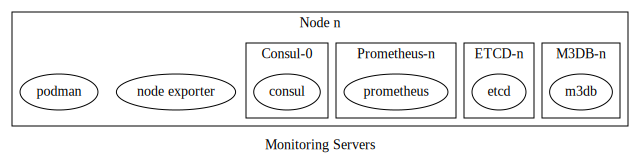
\includegraphics[width=16cm]{assets/node_configuration_diagram.png}
  \caption{Diagramm zur Übersicht eines Monitoringknotens}
  \label{figure:node}
\end{figure}

\begin{figure}[!htbp]
  \centering
  \includegraphics[width=16cm]{assets/netzwerkdiagramm.png}
  \caption{Diagramm zur Übersicht des Netzwerkes}
  \label{figure:network}
\end{figure}

\begin{figure}[!htbp]
  \centering
  \includegraphics[width=16cm]{assets/etcd_member_list.png}
  \caption{Ausgabe des ETCD zum Zustand des Cluster}
  \label{figure:member-list}
\end{figure}

\begin{figure}[!htbp]
  \centering
  \includegraphics[width=16cm]{assets/ansible_run_recap.png}
  \caption{Ausgabe der Zusammenfassung des Ansibleprozess}
  \label{figure:ansible-recap}
\end{figure}

\begin{figure}[!htbp]
  \centering
  \includegraphics[width=12cm]{assets/ansible_run_m3db.png}
  \caption{Ausgabe des Ansibleprozess}
  \label{figure:ansible-run}
\end{figure}

\begin{figure}[!htbp]
  \centering
  \includegraphics[width=16cm]{assets/m3db_grafana_dashboard.png}
  \caption{Grafana M3 Dashboard}
  \label{figure:m3-dash}
\end{figure}

\newpage

\begin{figure}[!htbp]
  \begin{lstlisting}
    [databse_servers]
    165.xxx.87.xxx
    161.xxx.213.xxx
    165.xxx.172.xxx
    \end{lstlisting}
  \caption{Beispiel für ein \gls{inventory} im \gls{INI}-Format}
  \label{figure:ansible-inv}
\end{figure}

\begin{figure}[!htbp]
  \begin{lstlisting}
  # HELP http_requests_total The total number of HTTP requests.
  # TYPE http_requests_total counter
  http_requests_total{method="post",code="200"} 678 1925066363000
  http_requests_total{method="post",code="400"}   1 1647066363000
  \end{lstlisting}
  \caption{Metricsformat Beispiel eines Webservers}
  \label{figure:metrics}
\end{figure}

\begin{figure}[!htbp]
  \begin{lstlisting}
  sum(rate(http_requests_total{job="prometheus"}[5d]))
  \end{lstlisting}
  \caption{
    \gls{promql} für die Summe aller \gls{http}-Request mit dem Label
    \emph{Prometheus} der letzten fünf Tage
  }
  \label{figure:promql}
\end{figure}

\begin{figure}[!htbp]
  \begin{lstlisting}
    ---
    - name: Postgres Playbook
      hosts: database_servers
      become: yes
      tasks:
      - name: ensure postgres is installed
        dnf:
          name: postgresql-server
          state: present
    \end{lstlisting}
  \caption{\glsadd{playbooks} Playbook zur Installation einer \emph{Postgres}-Datenbankmanagementsoftware}
  \label{figure:inv}
\end{figure}

\begin{figure}[!htbp]
  \begin{lstlisting}
    git init
    git remote add origin git@github.com:nk-designz/distributed_prometheus.git
  \end{lstlisting}
  \caption{Initialisierung des git-Repository mit \gls{remote} bei \emph{Github}}
  \label{figure:git}
\end{figure}

\begin{figure}[!htbp]
  \begin{lstlisting}
    ansible-galaxy init common
  \end{lstlisting}
  \caption{Initialisierung der \emph{common}-Rolle}
  \label{figure:galaxy}
\end{figure}

\begin{figure}[!htbp]
  \begin{lstlisting}
    ---
    - name: Setup Distributed Prometheus
      hosts: all
      become: yes
      remote_user: root
      roles:
      - cloudalchemy.node_exporter
    \end{lstlisting}
  \caption{\emph{main.yml} mit der \emph{NodeExporter}-Rolle}
  \label{figure:playbook}
\end{figure}

\begin{figure}[!htbp]
  \begin{lstlisting}
    ANSIBLE_HOST_KEY_CHECKING=false \
    ansible-playbook \
    -e 'ansible_python_interpreter=/usr/bin/python3' \
    -i inventory/hosts.ini \
    main.yml
  \end{lstlisting}
  \caption{Kommando zum Ausführen des \gls{playbooks}}
  \label{figure:ansible-command}
\end{figure}

\begin{figure}[!htbp]
  \begin{lstlisting}
    ansible.run:	inventory/hosts.ini
          ANSIBLE_HOST_KEY_CHECKING=false \
          ansible-playbook \
          -e 'ansible_python_interpreter=/usr/bin/python3' \
          -i inventory/hosts.ini \
          main.yml
  \end{lstlisting}
  \caption{Eintrag in der \gls{make}-Datei zum Ausführen des Projekts}
  \label{figure:make-ansible}
\end{figure}

\begin{figure}[!htbp]
  \begin{lstlisting}
    - name: Install common packages
      dnf:
        name: "{{ common_packages }}"
        state: present
  \end{lstlisting}
  \caption{Installation von allgemeinen Paketen}
  \label{figure:base-install}
\end{figure}

\begin{figure}[!htbp]
  \begin{lstlisting}
    # common packages for the nodes
    common_packages:
    - vim
    - htop
    - podman
    - firewalld
    - python3-firewall
    - jq
  \end{lstlisting}
  \caption{Allgemeine Pakete im \emph{defaults}-Verzeichnis}
  \label{figure:base-packages}
\end{figure}

\begin{figure}[!htbp]
  \lstinputlisting{../roles/requirements.yml}
  \caption{Externe \gls{rollen} in der \emph{requirements.yml}}
  \label{figure:requirements}
\end{figure}

\begin{figure}[!htbp]
  \begin{lstlisting}
    command: |
      /usr/local/bin/etcd
      --name {{ ansible_hostname }}
      --data-dir /var/run/etcd
      --advertise-client-urls http://{{ etcd_ip }}:2379,http://{{ etcd_ip }}:4001
      --listen-client-urls http://0.0.0.0:2379,http://0.0.0.0:4001
      --initial-advertise-peer-urls http://{{ etcd_ip }}:2380
      --listen-peer-urls http://0.0.0.0:2380
      --initial-cluster-token dont-use-this-token
      --initial-cluster {{ etcd_initial_cluster }}
      --initial-cluster-state new
      --data-dir /var/run/etcd
  \end{lstlisting}
  \caption{Ausschnitt aus dem Task zum Starten des ETCD-Container}
  \label{figure:etcd-command}
\end{figure}

\begin{figure}[!htbp]
  \begin{lstlisting}
    etcd_ip: "{{ hostvars[inventory_hostname]['ansible_default_ipv4']['address'] }}"
    etcd_initial_cluster: "{{ hostvars[host]['ansible_facts']['hostname'] }}=http://{{ hostvars[host]['ansible_facts']['eth0']['ipv4']['address'] }}:2380,"
    # etcd0=http://X.X.X.X:2380,etcd1=http://X.X.X.Y:2380,etcd2=http://X.X.X.Z:2380
  \end{lstlisting}
  \caption{Setzen der IP- und Clustervariablen aus den \emph{Absible Facts}}
  \label{figure:etcd-var}
\end{figure}

\begin{figure}[!htbp]
  \begin{lstlisting}
    volume:
    - /etc/m3dbnode:/etc/m3dbnode
    - /var/m3db:/var/lib/m3db
    - /var/m3kv:/var/lib/m3kv
    publish:
    - "7201:7201"
    - "7203:7203"
    - "9000:9000"
    - "9001:9001"
    - "9002:9002"
    - "9003:9003"
    - "9004:9004"
  \end{lstlisting}
  \caption{Ausschnitt des \gls{task} zum Start des \emph{m3db}-Containers}
  \label{figure:m3db-ports}
\end{figure}

\begin{figure}[!htbp]
  \lstinputlisting{../roles/m3db/templates/placement.json.j2}
  \caption{Template für die Payload zur \emph{Placement}-Konfiguration}
  \label{figure:m3db-placing}
\end{figure}

\begin{figure}[!htbp]
  \begin{lstlisting}
    global:
      scrape_interval: 15s
      evaluation_interval: 15s
    remote_write:
    - url: "http://localhost:7201/api/v1/prom/remote/write"
    scrape_configs:
    - job_name: 'consul_services'
    consul_sd_configs:
    - server: "127.0.0.1:8500"
      datacenter: "{{ consul_datacenter }}"
      scheme: http
      refresh_interval: "60s"
  \end{lstlisting}
  \caption{Ausschnitt aus der Prometheuskonfiguration}
  \label{figure:prometheus-conf}
\end{figure}

\newpage

% Tabellenverzeichnis
\listoftables
\newpage
\begin{table}[!htbp]
  \begin{tabular}{c l c c}
                             & Phasen        & Aufwand \emph{(Stunden)} & Kosten \emph{(EUR)} \\
    \hline
    \cellcolor[HTML]{FFF587} & Planung       & 5                        & 300                 \\
    \cellcolor[HTML]{FF8C64} & Realisierung  & 19                       & 1140                \\
    \cellcolor[HTML]{FF665A} & Evaluation    & 3                        & 180                 \\
    \cellcolor[HTML]{7D6B7D} & Dokumentation & 8                        & 480                 \\
    \hline
                             & Gesamt        & 35                       & 2.100               \\
  \end{tabular}
  \begin{tabular}{l c c}
    Ressource    & Anzahl & Kosten  \emph{(EUR)} \\
    \hline
    VServer      & 3      & 0                    \\
    Reverseproxy & 2      & 0                    \\
    \hline
    Gesamt       &        & 0
  \end{tabular}
  Ressourcen beim \gls{itz}
  \caption{Aufwandsschätzung aller Kosten bezogen auf die Projektphasen }
  \label{table:aufwand}
\end{table}

\begin{table}[!htbp]
  \begin{tabular}{l c | c c c c c}
    Abschnitte    & Stunden
                  & 1         & 2                        & 3                        & 4                        & 5                                                   \\
    \hline
    Durchführung der IST-Analyse
                  & \emph{1h} & \cellcolor[HTML]{FFF587} &                          &                          &                          &                          \\
    Ermittlung des Soll Zustands
                  & \emph{2h} & \cellcolor[HTML]{FFF587} &                          &                          &                          &                          \\
    Evaluierung der Spezifikation der VMs
                  & \emph{2h} & \cellcolor[HTML]{FFF587} &                          &                          &                          &                          \\
    Aufsetzen der Projektstruktur des Ansible Playbooks
                  & \emph{1h} & \cellcolor[HTML]{FF8C64} &                          &                          &                          &                          \\
    Konstruktion eines \gls{playbooks} zum Einrichtung des Monitorings
                  & \emph{2h} & \cellcolor[HTML]{FF8C64} &                          &                          &                          &                          \\
    Konstruktion einer\glsadd{rollen} Rolle für einen ETCD-Knoten
                  & \emph{3h} &                          & \cellcolor[HTML]{FF8C64} &                          &                          &                          \\
    Konstruktion einer\glsadd{rollen} Rolle für einen M3DB-Knoten
                  & \emph{4h} &                          & \cellcolor[HTML]{FF8C64} &                          &                          &                          \\
    Konstruktion einer\glsadd{rollen} Rolle für einen Consul-Knoten
                  & \emph{3h} &                          &                          & \cellcolor[HTML]{FF8C64} &                          &                          \\
    Konstruktion einer\glsadd{rollen} Rolle für einen Prometheus-Host
                  & \emph{3h} &                          &                          & \cellcolor[HTML]{FF8C64} &                          &                          \\
    Konstruktion einer\glsadd{rollen} Rolle für einen Grafana-Host
                  & \emph{2h} &                          &                          & \cellcolor[HTML]{FF8C64} &                          &                          \\
    Durchführung der Installation
                  & \emph{1h} &                          &                          &                          & \cellcolor[HTML]{FF8C64} &                          \\
    Eintragen von Betriebsdaten und Dashboards
                  & \emph{1h} &                          &                          &                          & \cellcolor[HTML]{FF665A} &                          \\
    Test der Monitoringlösung
                  & \emph{2h} &                          &                          &                          & \cellcolor[HTML]{FF665A} & \cellcolor[HTML]{FF665A} \\
    Dokumentation
                  & \emph{8h} & \cellcolor[HTML]{7D6B7D} & \cellcolor[HTML]{7D6B7D} & \cellcolor[HTML]{7D6B7D} & \cellcolor[HTML]{7D6B7D} & \cellcolor[HTML]{7D6B7D} \\
    \hline
    Tagesstunden  &           & 8h                       & 8h                       & 8h                       & 8h                       & 3h                       \\
    \hline
    Gesamtstunden &           &                          &                          & 35h                      &                          &                          \\
  \end{tabular}
  \caption{GANTT-Diagramm der Projektplanung}
  \label{table:gantt}
  \begin{tabular}{c l}
    \cellcolor[HTML]{FFF587} & Projektplanung \\
    \cellcolor[HTML]{FF8C64} & Realisierung   \\
    \cellcolor[HTML]{FF665A} & Evaluation     \\
    \cellcolor[HTML]{7D6B7D} & Dokumentation  \\
  \end{tabular}
  \captionof*{tabular}{Legende des GANTT-Diagramm}
\end{table}

\newpage
% Quellenverzeichnis
%\bibliographystyle{plain}
\begin{thebibliography}{9}

  \bibitem{bundesgesundheitsministerium}
  \texttt{\url{https://www.bundesgesundheitsministerium.de/}}
  \\\hfill \texttt{05.03.2021 8:43 Uhr}

  \bibitem{sormas-oegd}
  \texttt{\url{https://www.sormas-oegd.de/}}
  \\\hfill \texttt{05.03.2021 8:45 Uhr}

  \bibitem{itz}
  \texttt{\url{https://www.itzbund.de/}}
  \\\hfill \texttt{05.03.2021 9:21 Uhr}

  \bibitem{etcd}
  \texttt{\url{https://etcd.io/}}
  \\\hfill \texttt{09.03.2021 8:20 Uhr}

  \bibitem{raft}
  \texttt{\url{https://raft.github.io/raft.pdf}}
  \\\hfill \texttt{09.03.2021 8:33 Uhr}

  \bibitem{m3db}
  \texttt{\url{https://m3db.io}}
  \\\hfill \texttt{09.03.2021 15:02 Uhr}

  \bibitem{etcd-config}
  \texttt{\url{https://etcd.io/docs/v3.4/op-guide/configuration/}}
  \\\hfill \texttt{09.03.2021 9:40 Uhr}

  \bibitem{m3db-placement}
  \texttt{\url{https://m3db.io/docs/operational_guide/placement_configuration/}}
  \\\hfill \texttt{09.03.2021 16:01 Uhr}

  \bibitem{m3db-blog}
  \texttt{\url{https://eng.uber.com/m3/}}
  \\\hfill \texttt{09.04.2021 16:20 Uhr}

  \bibitem{m3db-vid}
  \texttt{\url{https://www.youtube.com/watch?v=CcH13GyszHI}}
  \\\hfill \texttt{09.04.2021 16:15 Uhr}

  \bibitem{cassandra}
  \texttt{\url{https://cassandra.apache.org/}}
  \\\hfill \texttt{05.03.2021 13:23 Uhr}

  \bibitem{split-brain}
  \texttt{\url{https://de.wikipedia.org/wiki/Split_Brain_(Informatik)}}
  \\\hfill \texttt{09.04.2021 15:32 Uhr}

  \bibitem{itz}
  \texttt{\url{https://www.itzbund.de/DE/home/home_node.html}}
  \\\hfill \texttt{09.04.2021 12:08 Uhr}


  \bibitem{sre}
  \texttt{\url{https://sre.google/sre-book/monitoring-distributed-systems/}}
  \\\hfill \texttt{09.04.2021 7:24 Uhr}

  \bibitem{go}
  \texttt{Introducing Go - Caleb Doxsey ISBN: 9781491941959}
  \\\hfill \texttt{2016}

  \bibitem{docker}
  \texttt{Docker - Sean P. Kane, Karl Matthias ISBN: 9781492036739}
  \\\hfill \texttt{2018}

  \bibitem{d2}
  \texttt{\url{https://www.youtube.com/watch?v=gqwcUgZOoyI}}
  \\\hfill \texttt{09.04.2021 14:08 Uhr}

  \bibitem{cap}
  \texttt{\url{https://www.ibm.com/cloud/learn/cap-theorem}}
  \\\hfill \texttt{09.03.2021 11:31 Uhr}

  \bibitem{prometheus}
  \texttt{\url{https://prometheus.io/docs/}}
  \\\hfill \texttt{14.03.2021 15:08 Uhr}

  \bibitem{exporter}
  \texttt{\url{https://prometheus.io/docs/instrumenting/exporters/}}
  \\\hfill \texttt{14.03.2021 16:22 Uhr}

  \bibitem{ms}
  \texttt{\url{https://microservices.io/}}
  \\\hfill \texttt{09.04.2021 14:17 Uhr}

  \bibitem{nosql}
  \texttt{\url{https://aws.amazon.com/de/nosql/}}
  \\\hfill \texttt{09.04.2021 11:00 Uhr}

  \bibitem{playbooks}
  \texttt{\url{https://docs.ansible.com/ansible/latest/user_guide/playbooks.html}}
  \\\hfill \texttt{09.04.2021 10:01 Uhr}

  \bibitem{ansible}
  \texttt{\url{https://www.ansible.com/resources/whitepapers/ansible-in-depth}}
  \\\hfill \texttt{09.04.2021 11:14 Uhr}

  \bibitem{grafana}
  \texttt{\url{https://grafana.com/docs/}}
  \\\hfill \texttt{09.04.2021 12:01 Uhr}

  \bibitem{podman}
  \texttt{\url{https://podman.io/}}
  \\\hfill \texttt{09.04.2021 10:01 Uhr}

  \bibitem{itil}
  \texttt{ITIL Foundation: ITIL 4 Edition - AXELOS ISBN: 9780113316144 }
  \\\hfill \texttt{2019}

\end{thebibliography}

\newpage
\appendix
% Anlagenseite
\begin{titlepage}
  \vspace*{1cm}
  \begin{center}
    {\bfseries\Huge
      \underline{Anlagen}\\
    }
    \Large
    \vspace{5cm}
    Genehmigter Projektantrag \\
    Bestätigung über die durchgeführte Projektarbeit
    \vfill
  \end{center}
\end{titlepage}

% Unterdrücken der Seitennummerierung
\thispagestyle{empty}
\pagenumbering{gobble}
\includepdf[link,pages=-,scale=1.0,pagecommand={}]{assets/Projektantrag.pdf}
\includepdf[link,pages=-,scale=1.0,pagecommand={}]{assets/projektbetaetigung.pdf}

\end{document}